\chapter{Identifying Best Performers}
\label{ch:identifying_best_performers}
% 1. Analyze performance results on different anomaly types per algorithm family
Starting out with the performance results from Schmidl et al. \cite{Schmidl2022} we deep dive into an analysis, comparing performance in different stages. In the first stage, the presented taxonomy is used to group the algorithms by families. We hypothesize that algorithm families show a significant correlation of their performance on different anomaly types. This hypothesis is primarily motivated by the families inherent characteristics, like SSA's focus on trend components. We test this hypothesis and use it to map algorithm structures to anomaly kinds, which can guide the algorithm selection process of future work. 

\section{Data Preprocessing}
% Filtering
In a first step, the performance results are filtered to evaluations that did not show any errors, which removes 22\% of the dataset.
Then we filter the dataset to research scope by removing multivariate input dimensionality and supervised algorithms, which further reduces the dataset by 60\%. In fact, after applying the input dimensionality filter, there are already no supervised algorithms left in the dataset, since Schmidl et al. \cite{Schmidl2022} did not evaluate univariate, supervised algorithms. This further supports the argument that labels are usually used to handle the complexity in multivariate cases.
During the whole filtering process, we make sure that no algorithms are dropped, only evaluation runs. Overall, the performance result dataset is reduced to 53\% of its original size, with 23849 results remaining.

% Augmentation with GutenTAG
In a second step, we augment the dataset with additional information about the time series used in evaluation. Such information is important for further analysis, which is why we add it to the evaluation results table. The algorithms were evaluated on real data from different datasets and on synthetic data, generated by the GutenTAG library \cite{Wenig2022}. The latter makes up 22\% of the whole performance result dataset (without the filtering from the first step). In order to follow the methodology and evaluate performance results against anomaly kinds, we augment the GutenTAG dataset with anomaly kinds. For each instance that was evaluated on the synthetic dataset, we want to know:
\begin{itemize}
    \item Does the time series contain multiple anomaly kinds (e.g. trend and mean)?
    \item What anomaly kind is present?
\end{itemize}
By doing so we can compare and analyze the evaluation results yielded on one specific kind of anomaly. Since in this case the data is synthetic we can formulate theses on their effect (e.g. does a certain algorithm excel on a certain anomaly type).

Within the GutenTAG dataset 76\% contain only one kind of anomaly (unique anomaly kind). Mapping the synthetic dataset's metadata to the performance results reveals that 75\% of the results performed on GutenTAG have unique anomalies. 
To conclude, 16\% (3932 entries) of the results after filtering were obtained on time series with known and unique anomaly kinds.

\section{Data Analysis}
A thorough data analysis is performed to better understand the results and identify possible biases.

\begin{figure}
    \centering
    % First Row of Subfigures
    \begin{subfigure}[b]{0.45\textwidth}
        \centering
        
\includegraphics[width=\textwidth]{plots/distribution_plots_pie_bar/bar_GutenTAG_tax.png}
        \subcaption{Algorithm Family}
        \label{fig:bar_GutenTAG_tax}
    \end{subfigure}
    \hfill
    \begin{subfigure}[b]{0.45\textwidth}
        \centering
        
\includegraphics[width=\textwidth]{plots/distribution_plots_pie_bar/bar_GutenTAG_anomaly.png}
        \subcaption{Anomaly Kind}
        \label{fig:bar_GutenTAG_anomaly}
    \end{subfigure}
   
    \caption{Dataset Proportions after Filtering based on different Measures.}
    \label{fig:GutenTag_dist}
\end{figure}

When comparing \ref{fig:GutenTag_dist} with Figure \ref{fig:overall_dist} we can see the effects of filtering... \todo{Figure side by side bar chart and comparison}

\paragraph{Hypothesis 1: Anomaly Nature and Characteristic influences Algorithm Performance} 
We hypothesize that an algorithm's performance is affected by the anomaly kind it is trying to detect. For instance, some could argue that algorithms with a smaller context size may have difficulties in identifying anomalies that occur over longer periods (trend anomaly). This is because their limited view might not capture the extended patterns of these long-duration anomalies effectively.

In order to test Hypothesis 1 we perform the above filtering and limit the evaluation results to the artificial GutenTAG dataset and exclusively use evaluation result that were yielded on time series with only one kind of anomaly. Finally, we compare the anomaly kind with performance values, grouped by the algorithm family. For grouping we use the taxonomy of Schmidl et al. \cite{Schmidl2022}. We also rely on the authors proposal to use \textit{Receiver Operating Characteristic Area Under the Curve} (ROC\_AUC) as a performance metric for comparison.

To test the hypothesis we use a two-way ANOVA. The results in Table \ref{tab:h1_anova} show a significant main effect for both, the anomaly kind and algorithm family variables on the dependent variable. This means that both variables influence the performance results significantly. We further discovered a significant interaction effect between anomaly kind and algorithm family, meaning that the kind of anomaly on the dependent variable varies depending on the algorithm family.

\begin{table}
\caption{ANOVA}
\label{tab:h1_anova}
\begin{tabular}{lrrrr}
\toprule
 & sum\_sq & df & F & PR(>F) \\
\midrule
\textbf{C(anomaly\_kind)} & 7.25 & 8.00 & 19.14 & 0.00 \\
\textbf{C(algo\_family)} & 23.60 & 5.00 & 99.77 & 0.00 \\
\textbf{C(anomaly\_kind):C(algo\_family)} & 12.21 & 40.00 & 6.45 & 0.00 \\
\textbf{Residual} & 183.47 & 3878.00 & NaN & NaN \\
\bottomrule
\end{tabular}
\end{table}


\paragraph{Hypothesis 2: Distinguishing Performance Results by Anomaly Type reveals the best-performing Algorithm Families.}
We argued that within the totality of algorithms, no best-performer can be identified. By using unique anomaly kinds and the taxonomy from Chapter \ref{ch:literature_review} we analyze the grouped performance results.

\begin{figure}
    \centering
    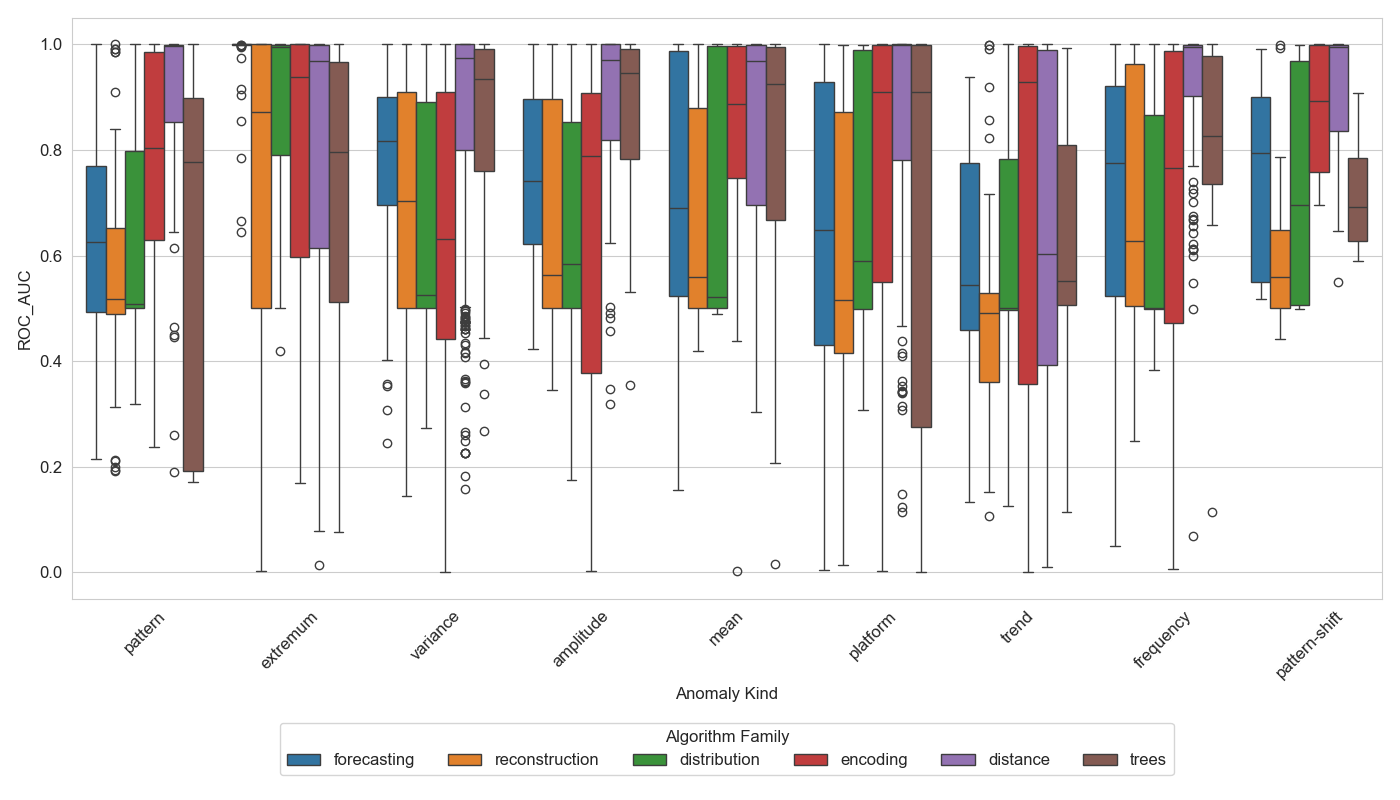
\includegraphics[width=1\textwidth]{plots/h1_boxplot_results.png}
    \caption{AUC-ROC Scores by Algorithm Family and Dataset}
    \label{fig:h1_boxplot_results}
\end{figure}

\begin{table}
\centering
\caption{Exact Values from Figure \ref{fig:h1_boxplot_results} with Mean Performance $> 0.8$}
\label{tab:best-performer}
\begin{tabular}{llrrr}
\toprule
 &  & count & mean & std \\
Anomaly Kind & Algorithm Family &  &  &  \\
\midrule
\multirow[t]{2}{*}{\textbf{amplitude}} & \textbf{distance} & 42 & 0.86 & 0.20 \\
\textbf{} & \textbf{trees} & 8 & 0.83 & 0.25 \\
\cline{1-5}
\multirow[t]{2}{*}{\textbf{extremum}} & \textbf{distribution} & 36 & 0.87 & 0.21 \\
\textbf{} & \textbf{forecasting} & 84 & 0.98 & 0.06 \\
\cline{1-5}
\multirow[t]{2}{*}{\textbf{frequency}} & \textbf{distance} & 125 & 0.92 & 0.14 \\
\textbf{} & \textbf{trees} & 24 & 0.83 & 0.20 \\
\cline{1-5}
\multirow[t]{2}{*}{\textbf{mean}} & \textbf{distance} & 82 & 0.85 & 0.20 \\
\textbf{} & \textbf{encoding} & 23 & 0.82 & 0.24 \\
\cline{1-5}
\textbf{pattern} & \textbf{distance} & 97 & 0.91 & 0.17 \\
\cline{1-5}
\multirow[t]{2}{*}{\textbf{pattern-shift}} & \textbf{distance} & 20 & 0.91 & 0.13 \\
\textbf{} & \textbf{encoding} & 6 & 0.87 & 0.14 \\
\cline{1-5}
\textbf{platform} & \textbf{distance} & 102 & 0.85 & 0.25 \\
\cline{1-5}
\multirow[t]{2}{*}{\textbf{variance}} & \textbf{distance} & 625 & 0.87 & 0.19 \\
\textbf{} & \textbf{trees} & 120 & 0.86 & 0.16 \\
\cline{1-5}
\bottomrule
\end{tabular}
\end{table}


Figure \ref{fig:h1_boxplot_results} reveals that there are differences in the mean performance values along different algorithm families per anomaly kind. Table \ref{tab:best-performer} shows the algorithm families with a mean performance value $>0.8$. We note that none of the algorithm families achieved this mean performance threshold on trend anomalies. The maximal mean performance on trend anomalies of $\sim 0.66$ was achieved by, both, distance and encoding algorithms.

The analysis highlights that distance-based methods stand out for their versatility, performing well across various anomaly types. This benefit is especially visible when capturing shifts in value and recurring patterns. 
Forecasting methods excel in extremum anomalies, showing the strengths of predictive models for significant deviations, such as sudden peaks or troughs. 
Tree methods are notably effective in handling amplitude, frequency and variance changes, while distribution-based methods perform best with extremum anomalies. Overall, distance-based methods provide robust, general performance, while other families like forecasting and distribution excel in more specific anomaly detection scenarios.

This analysis can already guide the choice of algorithms based on the specific anomaly types. Selecting algorithms from these families according to the anomaly kinds can yield optimized results in AD tasks on time series. However, Table \ref{tab:best-performer} shows variations in the standard deviation across all families, which asks for a deep-dive analysis within the families.


\section{Deep-Dive and Algorithm Analysis}
For each anomaly kind, we take a closer look at the performance results of each algorithm. The standard deviation in Figure \ref{fig:h1_boxplot_results} already revealed that within a best-performing family, some algorithms show bad performance. In the following, all algorithms within a best-performing family are compared to identify reasons why they outperformed or underperformed on a given anomaly kind. These results are formulated as hypotheses for internal structural advantages towards anomaly kinds. 

With distance methods being very prominent in this analysis, we first separate them further by their inherent structures and approaches to AD. The grouping in Table \ref{tab:distance_algos_structures} helps to simplify the analysis and retains a good overview.

\begin{table}[h!]
\centering
\caption{Grouping of Distance Algorithms by Structural Approach}
\label{tab:distance_algos_structures}
\begin{tabular}{ll}
\hline
\textbf{Structure/Approach} & \textbf{Algorithms} \\ \hline
\textbf{Model-Based} & NormA, SAND, SSA \\ 
\textbf{Symbolic and Pattern-Based} & HOT SAX, VALMOD \\
\textbf{Matrix Profile and Similarity-Based} & Left STAMPi, STOMP, STAMP \\
\textbf{Graph and Embedding-Based} & Series2Graph \\ 
\textbf{Density-Based} & Subsequence LOF \\ 
\textbf{SVM-Based and Hybrid Approaches} & PhaseSpace-SVM \\ \hline
\end{tabular}
\end{table}


\begin{itemize}
    \item \textbf{Model-Based}: Builds a model representing normal behavior, either through a predefined model (NormA) or adaptive, streaming updates (SAND, SSA). These algorithms detect anomalies as deviations from expected patterns.
    \item \textbf{Symbolic and Pattern-Based}: Utilizes symbolic representations or variable-length pattern recognition to identify unique or recurring subsequences. These methods focus on pattern distinctiveness and sometimes abstract details of fine variations.
    \item \textbf{Matrix Profile and Similarity-Based}: Employs matrix profiles to efficiently compute similarity joins. This structure allows to captures exact or near-exact patterns across large datasets.
    \item \textbf{Graph and Embedding-Based}: Represents time series data as a graph where nodes represent subsequences and edges indicate pattern transitions. 
    \item \textbf{Density-Based}: Detects anomalies based on local density measurements, identifying points that are isolated from their nearest neighbors.
    \item \textbf{SVM-Based and Hybrid Approaches}: Combines support vector machines with phase-space reconstruction to identify anomalies in temporal sequences, focusing on dynamic and nonlinear behaviors in time series data.
\end{itemize}


\subsection{Extremum Anomalies} 
    \begin{table}
\caption{Algorithms on extremum Anomaly within best-performing Family}
\label{tab:bp-extremum}
\begin{tabular}{llrrr}
\toprule
 &  & count & mean & std \\
Algorithm Family & Algorithm &  &  &  \\
\midrule
\multirow[t]{3}{*}{\textbf{distribution}} & \textbf{DSPOT} & 12 & 0.83 & 0.23 \\
\textbf{} & \textbf{DWT-MLEAD} & 12 & 0.94 & 0.11 \\
\textbf{} & \textbf{S-H-ESD (Twitter)} & 12 & 0.83 & 0.25 \\
\cline{1-5}
\multirow[t]{7}{*}{\textbf{forecasting}} & \textbf{ARIMA} & 12 & 0.89 & 0.13 \\
\textbf{} & \textbf{MedianMethod} & 12 & 1.00 & 0.00 \\
\textbf{} & \textbf{NumentaHTM} & 12 & 1.00 & 0.00 \\
\textbf{} & \textbf{OceanWNN} & 12 & 1.00 & 0.00 \\
\textbf{} & \textbf{Random Forest Regressor (RR)} & 12 & 1.00 & 0.00 \\
\textbf{} & \textbf{Triple ES (Holt-Winter's)} & 12 & 1.00 & 0.00 \\
\textbf{} & \textbf{XGBoosting (RR)} & 12 & 1.00 & 0.00 \\
\cline{1-5}
\bottomrule
\end{tabular}
\end{table}

    \textit{Forecasting} almost detected all extremum anomalies in testing, with ARIMA only missing a few.
    The adaptability to dynamic patterns of the MedianMethod, NumentaHTM and OceanWNN as well as the robustness through ensemble learning of RForest and XGBoosting seem to favor the detection of extremum anomalies. 
    ARIMA might struggle with non-linear or abrupt changes, which are typical in extremum anomalies. Its reliance on linear assumptions could limit its precision on complex, non-linear data patterns.
    
    \textit{Distribution} algorithms also performed reasonably well on extremum anomalies. DWT-MLEAD shows the best performance with highest consistency. The breakdown of the time series into multiple frequency components allows DWT-MLEAD to capture both short-term spikes and broader extremum patterns effectively, reflecting in the good overall performance. By additionally applying MLE on the decomposed data, DWT-MLEAD optimizes its thresholding, which likely reduces false positives (shown in its lower std dev of 0.11).
    DSPOT's dynamic threshold, being optimized for streaming data, adapts quickly. This might lead to a high sensitivity. Additionally, it does not decompose at multiple scales but instead applies its threshold across the entire dataset. If noise or frequent fluctuations are present, DSPOT might mistakenly classify these as extremum points, impacting its overall precision.
    S-H-ESD is robust to seasonality, which might make it less effective for unpredictable extremum anomalies that fall outside seasonal expectations.

\subsection{Frequency Anomalies}
    \begin{table}
\caption{Algorithms on frequency Anomaly within best-performing Family}
\label{tab:bp-frequency}
\begin{tabular}{llrrrrrrrr}
\toprule
 &  & count & mean & std & min & 25\% & 50\% & 75\% & max \\
Algorithm Family & Algorithm &  &  &  &  &  &  &  &  \\
\midrule
\multirow[t]{11}{*}{\textbf{distance}} & \textbf{HOT SAX} & 5.00 & 0.80 & 0.20 & 0.50 & 0.73 & 0.83 & 0.97 & 1.00 \\
\textbf{} & \textbf{Left STAMPi} & 12.00 & 0.98 & 0.04 & 0.89 & 0.98 & 1.00 & 1.00 & 1.00 \\
\textbf{} & \textbf{NormA} & 12.00 & 1.00 & 0.01 & 0.98 & 1.00 & 1.00 & 1.00 & 1.00 \\
\textbf{} & \textbf{PhaseSpace-SVM} & 12.00 & 0.95 & 0.06 & 0.82 & 0.90 & 0.99 & 1.00 & 1.00 \\
\textbf{} & \textbf{SAND} & 12.00 & 0.99 & 0.01 & 0.97 & 0.99 & 1.00 & 1.00 & 1.00 \\
\textbf{} & \textbf{SSA} & 12.00 & 0.71 & 0.14 & 0.55 & 0.61 & 0.66 & 0.76 & 1.00 \\
\textbf{} & \textbf{STAMP} & 12.00 & 0.97 & 0.06 & 0.81 & 0.98 & 1.00 & 1.00 & 1.00 \\
\textbf{} & \textbf{STOMP} & 12.00 & 0.97 & 0.06 & 0.81 & 0.98 & 1.00 & 1.00 & 1.00 \\
\textbf{} & \textbf{Series2Graph} & 12.00 & 0.87 & 0.27 & 0.07 & 0.89 & 0.99 & 1.00 & 1.00 \\
\textbf{} & \textbf{Subsequence LOF} & 12.00 & 0.94 & 0.13 & 0.67 & 0.99 & 1.00 & 1.00 & 1.00 \\
\textbf{} & \textbf{VALMOD} & 12.00 & 0.90 & 0.15 & 0.61 & 0.80 & 0.99 & 1.00 & 1.00 \\
\cline{1-10}
\multirow[t]{2}{*}{\textbf{trees}} & \textbf{PST} & 12.00 & 0.92 & 0.11 & 0.66 & 0.93 & 0.97 & 0.99 & 1.00 \\
\textbf{} & \textbf{Subsequence IF} & 12.00 & 0.73 & 0.22 & 0.11 & 0.73 & 0.75 & 0.77 & 1.00 \\
\cline{1-10}
\bottomrule
\end{tabular}
\end{table}

    Within the \textit{distance} family, two model-based methods NormA and SAND achieved the highest means ($0.997$ and $0.993$) with very low variance. However, SSA yields the lowest performance of all distance methods. This does not generally speak in favor of model-based structures towards frequency anomalies, but, SSA is build around seasonal and trend components. It might overly rely on these components, leading to bad performance in frequency anomalies.
    The matrix-profile and similarity based approaches overall show high mean performance with small standard deviations. This inherent structure excels at identifying repeated sequences, probably leading to the high performance on frequency anomalies.
    The rest shows moderate to high performance with no indication on structural advantages.
    
    PST from the \textit{tree} family achieves comparable results. It likely outperforms Subsequence IF due to its focuses on encoding frequent patterns with suffix trees. By capturing these patterns probabilistically, it is better suited to recognize anomalies as any deviation in the frequency of expected patterns, which is ideal for detecting frequency anomalies. Subsequence IF does not inherently focus on frequency anomalies but isolates points independently, which may produce false positives or miss certain frequency-related anomalies.
    
\subsection{Mean Anomalies} 
    \begin{table}[h]
\centering
\caption{Algorithms on Mean Anomaly within best-performing Family}
\label{tab:bp-mean}
\begin{tabular}{llrrr}
\toprule
 &  & count & mean & std \\
Algorithm Family & Algorithm &  &  &  \\
\midrule
\multirow[t]{11}{*}{\textbf{distance}} & \textbf{HOT SAX} & 3 & 0.85 & 0.21 \\
\textbf{} & \textbf{Left STAMPi} & 8 & 0.83 & 0.28 \\
\textbf{} & \textbf{NormA} & 8 & 0.88 & 0.23 \\
\textbf{} & \textbf{PhaseSpace-SVM} & 8 & 0.73 & 0.17 \\
\textbf{} & \textbf{SAND} & 7 & 0.96 & 0.05 \\
\textbf{} & \textbf{SSA} & 8 & 0.80 & 0.16 \\
\textbf{} & \textbf{STAMP} & 8 & 0.90 & 0.24 \\
\textbf{} & \textbf{STOMP} & 8 & 0.90 & 0.24 \\
\textbf{} & \textbf{Series2Graph} & 8 & 0.92 & 0.12 \\
\textbf{} & \textbf{Subsequence LOF} & 8 & 0.94 & 0.09 \\
\textbf{} & \textbf{VALMOD} & 8 & 0.67 & 0.20 \\
\cline{1-5}
\multirow[t]{3}{*}{\textbf{encoding}} & \textbf{GrammarViz} & 8 & 0.98 & 0.04 \\
\textbf{} & \textbf{TARZAN} & 7 & 0.70 & 0.37 \\
\textbf{} & \textbf{TSBitmap} & 8 & 0.77 & 0.14 \\
\cline{1-5}
\bottomrule
\end{tabular}
\end{table}

    Looking back at Table \ref{tab:best-performer} we see only a small difference, between the two best-performing families distance and encoding, on mean anomalies.
    Overall, the \textit{distance} family does not show a high variablilty in performance between different algorithms. All algorithms show moderate to high performance mean with PhaseSpace-SVM and VALMOD being the exception. This does not align with the structural grouping from Table \ref{tab:distance_algos_structures} and needs further analysis of the two algorithms. Both PhaseSpace-SVM and VALMOD are optimized for detecting distinct or abrupt anomalies tied to structural or temporal patterns rather than gradual shifts in central tendency. PhaseSpace-SVM focuses on temporal evolution, making it more suited to dynamic anomalies, while VALMOD searches distinctive motifs or isolated discords. Both approaches do not align well with the characteristics of mean anomalies.
    
    A similar concept could explain the deviations in the \textit{encoding} family. GrammarViz clearly outperforms TARZAN and TSBitmap. GrammarViz’s identifies deviations from common rules, its grammar, which makes it well-suited for detecting gradual changes in central tendency. TARZAN uses a suffix tree combined with a Markov model to detect surprising patterns, while TSBitmap focuses on visual pattern detection. Both approaches might hinder the performance on gradual changes.
    
\subsection{Pattern Anomalies}
    \begin{table}
\caption{Algorithms on pattern Anomaly within best-performing Family}
\label{tab:bp-pattern}
\begin{tabular}{llrrr}
\toprule
 &  & count & mean & std \\
Algorithm Family & Algorithm &  &  &  \\
\midrule
\multirow[t]{11}{*}{\textbf{distance}} & \textbf{HOT SAX} & 7 & 0.76 & 0.30 \\
\textbf{} & \textbf{Left STAMPi} & 9 & 0.95 & 0.10 \\
\textbf{} & \textbf{NormA} & 9 & 0.96 & 0.10 \\
\textbf{} & \textbf{PhaseSpace-SVM} & 9 & 0.90 & 0.13 \\
\textbf{} & \textbf{SAND} & 9 & 0.96 & 0.08 \\
\textbf{} & \textbf{SSA} & 9 & 0.79 & 0.28 \\
\textbf{} & \textbf{STAMP} & 9 & 0.94 & 0.12 \\
\textbf{} & \textbf{STOMP} & 9 & 0.94 & 0.12 \\
\textbf{} & \textbf{Series2Graph} & 9 & 0.92 & 0.18 \\
\textbf{} & \textbf{Subsequence LOF} & 9 & 0.97 & 0.05 \\
\textbf{} & \textbf{VALMOD} & 9 & 0.86 & 0.20 \\
\cline{1-5}
\bottomrule
\end{tabular}
\end{table}

    Distance based approaches appear to capture pattern anomalies the best, with most  algorithms achieving high performance results. SSA and HOT SAX strike with lower mean performance and the highest standard deviation.
    With VALMOD performing well but also lower than average (mean of $0.91$ across all anomaly kinds) symbolic and pattern-based approaches appear to underperform on pattern anomalies, contrary to their original idea. Depending on the scale of abnormality, this could be explained by their level of abstraction, which can lead to a lower sensitivity.
    The bad performance of SSA could, again, be explained by its assumption of inherent seasonal and trend components.
    
\subsection{Pattern Shift Anomalies}
    \begin{table}
\caption{Algorithms on pattern-shift Anomaly within best-performing Family}
\label{tab:bp-pattern-shift}
\begin{tabular}{llrrr}
\toprule
 &  & count & mean & std \\
Algorithm Family & Algorithm &  &  &  \\
\midrule
\multirow[t]{10}{*}{\textbf{distance}} & \textbf{Left STAMPi} & 2 & 1.00 & 0.00 \\
\textbf{} & \textbf{NormA} & 2 & 1.00 & 0.00 \\
\textbf{} & \textbf{PhaseSpace-SVM} & 2 & 0.84 & 0.04 \\
\textbf{} & \textbf{SAND} & 2 & 1.00 & 0.00 \\
\textbf{} & \textbf{SSA} & 2 & 0.73 & 0.26 \\
\textbf{} & \textbf{STAMP} & 2 & 1.00 & 0.00 \\
\textbf{} & \textbf{STOMP} & 2 & 1.00 & 0.00 \\
\textbf{} & \textbf{Series2Graph} & 2 & 0.82 & 0.25 \\
\textbf{} & \textbf{Subsequence LOF} & 2 & 0.84 & 0.05 \\
\textbf{} & \textbf{VALMOD} & 2 & 0.83 & 0.01 \\
\cline{1-5}
\multirow[t]{3}{*}{\textbf{encoding}} & \textbf{GrammarViz} & 2 & 1.00 & 0.00 \\
\textbf{} & \textbf{TARZAN} & 2 & 0.85 & 0.21 \\
\textbf{} & \textbf{TSBitmap} & 2 & 0.77 & 0.03 \\
\cline{1-5}
\bottomrule
\end{tabular}
\end{table}

    Here, the \textit{distance} family shows a similar picture. SSA seems to struggle with handling pattern-shift anomalies due to missing seasonal and trend components, while the other model-based approaches outperform.
    Matrix profile and similarity based algorithms excel on pattern-shift anomalies. As they can continuously compare subsequences across the time series they are sensitivity to changes in similarity allowing them to effectively catch pattern shifts.

    For \textit{encoding} algorithms, we follow the hypothesis formulated for mean anomalies, to explain the bad performance of TARZAN and TSBitmap. The same goes for GrammarViz. Its established grammar is broken by pattern shifts, which introduce deviations in sequence or timing, probably making it efficient on pattern-shifts.
    
\subsection{Platform Anomalies}
    \begin{table}[h]
\centering
\caption{Algorithms on Platform Anomaly within best-performing Family}
\label{tab:bp-platform}
\begin{tabular}{llrrr}
\toprule
 &  & count & mean & std \\
Algorithm Family & Algorithm &  &  &  \\
\midrule
\multirow[t]{11}{*}{\textbf{distance}} & \textbf{HOT SAX} & 5 & 0.76 & 0.35 \\
\textbf{} & \textbf{Left STAMPi} & 10 & 0.93 & 0.21 \\
\textbf{} & \textbf{NormA} & 10 & 0.91 & 0.20 \\
\textbf{} & \textbf{PhaseSpace-SVM} & 10 & 0.83 & 0.28 \\
\textbf{} & \textbf{SAND} & 10 & 0.93 & 0.15 \\
\textbf{} & \textbf{SSA} & 10 & 0.67 & 0.27 \\
\textbf{} & \textbf{STAMP} & 10 & 0.93 & 0.21 \\
\textbf{} & \textbf{STOMP} & 10 & 0.93 & 0.21 \\
\textbf{} & \textbf{Series2Graph} & 9 & 0.82 & 0.34 \\
\textbf{} & \textbf{Subsequence LOF} & 10 & 0.69 & 0.23 \\
\textbf{} & \textbf{VALMOD} & 8 & 0.92 & 0.23 \\
\cline{1-5}
\bottomrule
\end{tabular}
\end{table}

    Model-based and matrix profile and similarity-based algorithms show high performance throughout, with SSA being the exception possible due to the missing trend and seasonality components.
    Almost all other approaches only achieve moderate performance on platform anomalies. Strikingly, VALMOD achieves good performance with moderate standard deviation within the rest. In platform anomalies, where the data holds a new baseline over a prolonged period, the motif and discord discovery might capture the new levels in the time series as distinct patterns. This could be seen as a structural advantage on platform anomalies.
    
\subsection{Variance Anomalies}
    \begin{table}
\caption{Algorithms on variance Anomaly within best-performing Family}
\label{tab:bp-variance}
\begin{tabular}{llrrr}
\toprule
 &  & count & mean & std \\
Algorithm Family & Algorithm &  &  &  \\
\midrule
\multirow[t]{11}{*}{\textbf{distance}} & \textbf{HOT SAX} & 47 & 0.78 & 0.20 \\
\textbf{} & \textbf{Left STAMPi} & 60 & 0.89 & 0.16 \\
\textbf{} & \textbf{NormA} & 50 & 0.72 & 0.25 \\
\textbf{} & \textbf{PhaseSpace-SVM} & 60 & 0.97 & 0.05 \\
\textbf{} & \textbf{SAND} & 49 & 0.88 & 0.17 \\
\textbf{} & \textbf{SSA} & 60 & 0.75 & 0.21 \\
\textbf{} & \textbf{STAMP} & 60 & 0.90 & 0.17 \\
\textbf{} & \textbf{STOMP} & 60 & 0.90 & 0.17 \\
\textbf{} & \textbf{Series2Graph} & 59 & 0.87 & 0.17 \\
\textbf{} & \textbf{Subsequence LOF} & 60 & 0.97 & 0.07 \\
\textbf{} & \textbf{VALMOD} & 60 & 0.91 & 0.16 \\
\cline{1-5}
\multirow[t]{2}{*}{\textbf{trees}} & \textbf{PST} & 60 & 0.87 & 0.18 \\
\textbf{} & \textbf{Subsequence IF} & 60 & 0.86 & 0.15 \\
\cline{1-5}
\bottomrule
\end{tabular}
\end{table}

    The \textit{distance} family reveals a different picture on variance anomalies. While performing well on other anomaly types, NormA marks the worst mean performance value here. The reason might be its reliance on detecting changes in the central tendency. Changes in data spread, like variance anomalies, do not align with this focus, thus, potentially leading to the bad performance.
    PhaceSpace-SVM, on the other hand, achieves a higher performance than its mean across all anomaly kinds. Its phase-space reconstruction seems to captures dynamic, variance-based changes in data more reliably than a stable central model. The SVM possibly enhances this by identifying boundary deviations, which are characteristic of variance anomalies. 
    It has to be noted that, as indicated by the counts in Table \ref{tab:bp-variance} and seen in Figure \ref{fig:distribution_chart}, the most samples were used in the evaluation on this anomaly type.
    
\subsection{Trend Anomalies} 
    As noted above, none of the algorithm families achieved mean performance threshold on trend anomalies. We break our methodology to identify best-performers across all families.
    \begin{table}[h]
\centering
\caption{Individual Algorithm Performance Analysis on Trend Anomalies.}
\label{tab:bp-trend}
\begin{tabular}{llrrr}
\toprule
 &  & count & mean & std \\
Algorithm Family & Algorithm &  &  &  \\
\midrule
\textbf{distance} & \textbf{Subsequence LOF} & 5.00 & 0.86 & 0.29 \\
\cline{1-5}
\textbf{distribution} & \textbf{DWT-MLEAD} & 5.00 & 0.82 & 0.39 \\
\cline{1-5}
\multirow[t]{2}{*}{\textbf{encoding}} & \textbf{GrammarViz} & 5.00 & 0.91 & 0.21 \\
\textbf{} & \textbf{TSBitmap} & 5.00 & 0.83 & 0.28 \\
\cline{1-5}
\bottomrule
\end{tabular}
\end{table}
    Table \ref{tab:bp-trend} reveals that encoding methods perform well on trend anomalies but were not considered because of the destructive performance result of TARZAN of $0.13$. This significant difference in the performance results within one family can be explained by TARZAN's inherent focus on discrete, unexpected patterns. GrammarViz’s grammar-based approach detects shifts in established patterns, while TSBitmap’s visual representation highlights progressive changes. A similar focus that is set by Subsequence LOF, which together make up the highest mean performance values on trend anomalies. 
    Interestingly, SSA only achieved a mean performance of $0.65$ on trend anomalies, which is incompatible with our hypothesis that it excels on time series with trend and seasonal components. 



% Challenges and Solutions
% Code Snippets 